\documentclass[solution,addpoints,12pt]{exam}
\printanswers
\usepackage{amsmath,amssymb}
\usepackage{multirow}
\usepackage{enumitem}
\usepackage[colorlinks=true, linkcolor=blue, urlcolor=blue]{hyperref}
\newcommand{\RP}{\ensuremath{\mathsf{RP}}}
\newcommand{\expect}[1]{\ensuremath{\mathbb{E}[#1]}}
\newcommand{\dx}{\mathrm{d}x}
\usepackage{graphicx}
\pointpoints{mark}{marks}

\begin{document}

\hrule
\vspace{1mm}
\noindent 
\begin{center}
{\Large CS6700 : Reinforcement Learning} \\
{\large Written Assignment \#3}
\end{center}
%\hfill Release date: 21 Jan, 2017, 12:00 pm}
\vspace{1mm}
\noindent 
{\large \hfill Deadline: ??}

\vspace{2mm}
\hrule

{\small

\begin{itemize}\itemsep0mm
\item This is an individual assignment. Collaborations and discussions are strictly
prohibited.
\item Be precise with your explanations. Unnecessary verbosity will be penalized.
\item Check the Moodle discussion forums regularly for updates regarding the assignment.
\item \textbf{Please start early.}
%\item Turn in \textbf{only the answers} on Turnitin.
\end{itemize}
}

\hrule

\vspace{3mm}
\noindent {\sc Author :} Rahul Reddy V \\[1mm]
\noindent {\sc Roll Number :} ME16B171   \\
%\hrule


\begin{questions}
\question[3] Consider the problem of solving POMDPs using Deep Reinforcement Learning. Can you think of ways to modify the standard DQN architecture to ensure it can remember histories of states. Does the experience replay also need to be modified? Explain.

\begin{solution}
Instead of solving the POMDP, we can solve an MDP with the belief state space of the POMDP as the new state space. Since we are now working with belief states we don't have to remember the histories of states. Instead we can just store the <b, a, r, b'> tuples in experience replay. However since the belief state space is continous and very high-dimensional based on the state space of the POMDP this approach would be computationally expensive. 
\end{solution}


\question[4] Exploration is often ameliorated by the use of counts over the various states. For example, one could maintain a visitation count $N(s)$, for every state and use the same to generate an intrinsic reward ($r_i(s)$) for visiting that state.
\[ r_i(s) = \tau \times \frac{1}{N(s)} \]
However, it is intractable to maintain these counts in high-dimensional spaces, since the count values will be zero for a large fraction of the states. Can you suggest a solution(s) to handle this scenario? How can you maintain an approximation of the counts for a large number of states and possibly generalize to unseen states?

\begin{solution}
The high dimensional state space can be discretized with the help a hash function and then the visitation counts for each of these hash codes can be maintained. \\
However the performance of this exploration method highly depends on the hash function used and the granularity of it. A popular hash function class for this task is locality-sensitive hashing(LSH) which groups similar states into one hash code and keeps distant states seperate. So, this method generalises well to states unseen before if a good hash function is chosen. 
\end{solution}

\question[5] Suppose that the MDP defined on the observation space is k-th order Markov, i.e. remembering the last k observations is enough to predict the future. 
Consider using a belief state based approach for solving this problem. For any starting state and initial belief, the belief distribution will localize to the right state after k updates, i.e., the true state the agent is in will have a probability of 1 and the other states will have a probability of 0. Is this statement true or false? Explain your answer. 

\begin{solution}
False. If the belief state is randomly initialized and the environment reset state(goal state) is reached within k steps, the belief state won't localize to the true state with probability 1 as the states before the reset state are useless. And also the observations have to be error free for the belief to localize to true state with probability 1.  
\end{solution}

\question[3]
Q-MDPs are a technique for solving the problem of behaving in POMDPs. The behavior produced by this approximation would not be optimal. In what sense is it not optimal?  Are there circumstances under which it can be optimal?

\begin{solution}
In Q-MDP approach to solving the problem of behaving in a POMDP, we assume that there is an underlying MDP and we know its optimal state-action value function($Q^{*}$), and we estimate the Q function for the belief states by taking a weighted average of the MDP state-action values.
\begin{equation}
 Q(b, a) = \sum_{s} b(s) Q^{*}(s, a)
\end{equation}
Though the Q function used is optimal for the fully known MDP, it's not optimal for the POMDP as we don't know the state we are in exactly and Q-MDP approach doesn't take that into consideration. The optimal policy would consider the partial observability.\\
Q-MDP would be optimal under the circumstances of all belief states being very close to the true state.
\end{solution}

\question[3] What are some advantages and disadvantages of A3C over DQN? What are some potential issues that can be caused by asynchronous updates in A3C?

\begin{solution}
\begin{itemize}
 \item \textbf{Adavantages of A3C over DQN:}
    \begin{itemize}
     \item A3C uses multiple workers sampling data simultaneously using different CPU threads, so it can get more data in less time compared to DQN(less training time).
     \item Using multiple agents exploring different parts of the environment with possibly different exploration strategies which produce de-correlated samples. This eliminates need of experience replay which is present in DQN and is computationally expensive.
     \item A3C can use both on-policy and off policy methods whereas DQN can only use off policy methods.
    \end{itemize} 
\end{itemize}

\begin{itemize}
 \item \textbf{Disadvantages of A3C over DQN:}
    \begin{itemize}
     \item Because the updates are done in asynchronous manner, different workers would update the same global network at different times, some workers might be computing the updates using an older version of global network but the global network was already changed by other workers. This could lead to reduce in performance. This is a potential issue due to asynchronous updates in A3C
    \end{itemize} 
\end{itemize}

\end{solution}

\question[6] There are a variety of very efficient heuristics available for solving deterministic travelling salesman problems. We would like to take advantage of such heuristics in solving
certain classes of large scale navigational problems in stochastic domains. These problems involve navigating from one well demarcated region to another. For e.g., consider
the problem of delivering mail to the office rooms in a multi storey building.

\begin{parts}
    \part[4] Outline a method to achieve this, using concepts from hierarchical RL.
    \begin{solution}
    The objective of this problem is to minimize the overall cost(time taken or distance covered) while delivering mail to the office rooms in a multi storey building without visiting any room more than once. One approach to solve thhis problem is to set sub tasks such as "Go to nth Floor", "Go to office room A" etc and learn option policies to these sub tasks. After learning these options, approriate positive rewards can be set for delivering mail and negative rewards for re-visiting an office room and a small negative reward for each step. With this all setup, now we can train the agent to solve the problem using Intra Option Q-Learning or SMPD Q-learning.  
    \end{solution}
    \part[2] What problems would such an approach encounter?
    \begin{solution}
    Since mails are stochastic, there might not be any mails to deliver to a certain room while training the agent but after deployment there could be mails to that room. Changes in the external distributions can affect the agent heavily. Since the agent has to make a round trip back to the initial position after delivering all the mails, It might skip few deliveries at times and return to initial position before.
    \end{solution}
\end{parts}

\question[6] This question may require you to refer to \href{this}{https://link.springer.com/content/pdf/10.1007/BF00114727.pdf} paper on average reward RL. Consider the 3 state MDP shown in Figure \ref{fig:avg}.  Mention the recurrent class for each such policies. In the average reward setting, what are the corresponding $\rho^{\pi}$ for each such policy ? Furthermore, which of these policies are gain optimal ? 
    \begin{parts}
        \part[3] What are the different deterministic uni-chain policies present ?
        \begin{solution}
        The different deterministic uni-chain policies present are:
        \begin{enumerate}
         \item $\pi_{1}(A) = a_{1};\; \pi_{1}(B) = a_{1};\; \pi_{1}(C) = a_{2}$; \\
          recurrent class of $\pi_{1} :\{A,B\}$
          
          \item $\pi_{2}(A) = a_{2};\; \pi_{1}(B) = a_{1};\; \pi_{1}(C) = a_{2}$; \\
          recurrent class of $\pi_{2} :\{A,C\}$
          
          \item $\pi_{3}(A) = a_{3};\; \pi_{1}(B) = a_{1};\; \pi_{1}(C) = a_{2}$; \\
          recurrent class of $\pi_{3} :\{A,C\}$
          
          \item $\pi_{4}(A) = a_{2};\; \pi_{1}(B) = a_{1};\; \pi_{1}(C) = a_{3}$; \\
          recurrent class of $\pi_{4} :\{C\}$
          
          \item $\pi_{5}(A) = a_{3};\; \pi_{1}(B) = a_{1};\; \pi_{1}(C) = a_{3}$; \\
          recurrent class of $\pi_{5} :\{C\}$
        \end{enumerate}

        \end{solution}
        \part[3] In the average reward setting, what are the corresponding $\rho^{\pi}$ for each such policy ? Furthermore, which of these policies are gain optimal ? 
        \begin{solution}
        \begin{enumerate}
         \item $\rho^{\pi_{1}} = 1$
         \item $\rho^{\pi_{2}} = 0.5$
         \item $\rho^{\pi_{3}} = 0$
         \item $\rho^{\pi_{4}} = 1$
         \item $\rho^{\pi_{5}} = 1$
        \end{enumerate}
        The gain optimal policies are $\pi_{1},\pi_{4},\pi_{5}$
        \end{solution}
    \end{parts}

    \begin{figure}[h]
        \centering
        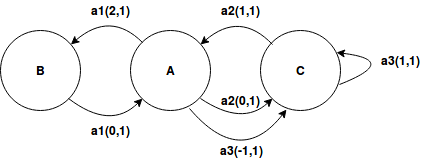
\includegraphics[scale=0.6]{average_reward.png}
        \caption{Notation : action(reward, transition probability). Example : a1(3, 1) refers to action a1 which results in a transition with reward +3 and probability 1}
        \label{fig:avg}
    \end{figure}

\end{questions}


\end{document}
